%% Short data paper template
%% Created by Simon Hengchen and Nilo Pedrazzini for the Journal of Open Humanities Data (https://openhumanitiesdata.metajnl.com)

\documentclass[11pt]{article}
\usepackage[english]{babel}
\usepackage[utf8]{inputenc}
\usepackage{johd}
\usepackage{ragged2e}
\usepackage{array}


\begin{document}

\thispagestyle{empty}
%%%%%%%%%%   Edit the thesis title here   %%%%%%%%%%


\begin{figure}[!h]
\centering

\includegraphics{uzh_logo.pdf}\\\
\end{figure}
\vspace{1cm}

\begin{center}
\huge {Cryptocurrencies and the risk-free rate}
\end{center}
\vspace{1cm}

\begin{center}
\large \textbf{Final Project}\\
\vspace{0.5cm}
Digital Tools for Finance (L) (03SMDFOEC008)\\
Department of Banking and Finance, University of Zurich\\
Igor Pozdeev
\end{center}
\vspace{1cm}

\begin{center}
\large \textbf{Authors}\\
\vspace{0.5cm}
Jakob Pirs (XX-XXX-XX, jakob.pirs@uzh.ch)\\

Nina Erminia Cantoni (17-709-221, ninaerminia.cantoni@uzh.ch)\\

Rohit Koonireddy (XX-XXX-XX, rohit.koonireddy@bf.uzh.ch)\\

Yunxiang Guo (XX-XXX-XX, yunxiang.guo@uzh.ch)\\
\end{center}
\vspace{1cm}

\begin{center}
\large \textbf{Abstract}\\
\vspace{0.5cm}
\begin{justify}
tbd
\end{justify}
\end{center}
\vspace{1cm}


\begin{center}
\vfill{}
\par\end{center}

\begin{center}
\renewcommand{\today}{\ifcase \month \or January\or February\or March\or   April\or May \or June\or July\or August\or September\or October\or November\or  December\fi, \number \year} 

\begin{center}
\large{\today}
\end{center}
\end{center}

\pagebreak{}
\pagebreak{}


\setcounter{page}{1}
\section{Context and motivation}


The goal of this paper is to analyze the correlation between the 10 year treasury yield and cryptocurrencies. The 10 year treasury rate is the yield one receives for investing in US government securities with a maturity of 10 years. It is a common proxy for the risk free rate. The risk free rate is a basic component of most pricing theories and thus a very relevant factor in the finance world. This paper will shed light on the influence of the risk free rate on the price of cryptocurrencies by analyzing price data over a period of 5 years. It will also be examined, wether the cryptocurrency market as a whole is affected.
\\

To answer our research question we look at four different cryptocurrencies, namely Bitcoin, Etherium,  XRP (by Ripple) and Litecoin. Find an overview of the four currencies in Table 1 below.


\begin{table}[H]
\centering % Label your table accordingly
\begin{tabular}{>{\centering\arraybackslash}m{0.15\textwidth} >{\centering\arraybackslash}m{0.15\textwidth} >{\centering\arraybackslash}m{0.15\textwidth} >{\centering\arraybackslash}m{0.15\textwidth} >{\centering\arraybackslash}m{0.15\textwidth}}
\hline
Logo & Name & Symbol & Market Cap as of Nov 25, 2022 & Ranking as of Nov 25, 2022\\
\hline
\\
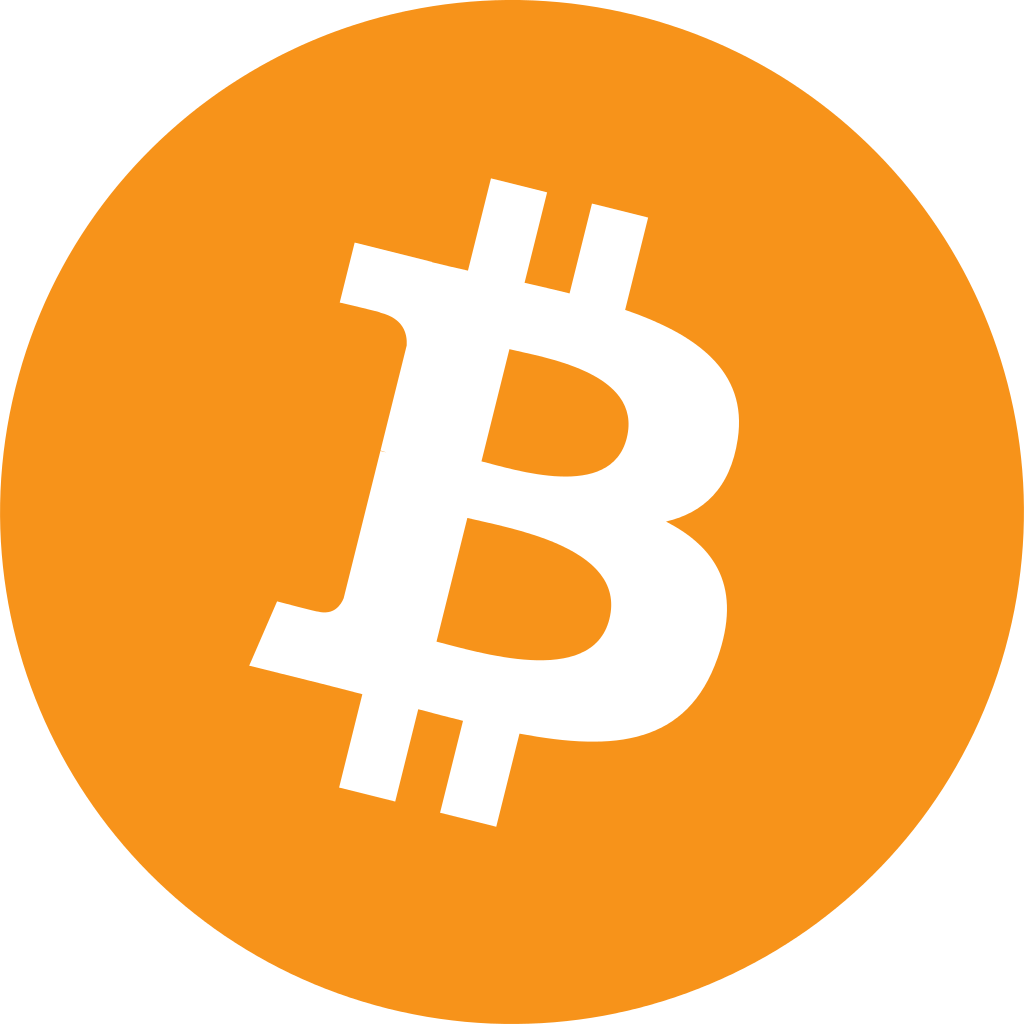
\includegraphics[width=0.1\textwidth]{Bitcoin.png} &  Bitcoin & BTC & \$ 318 bn & 1\\
\\
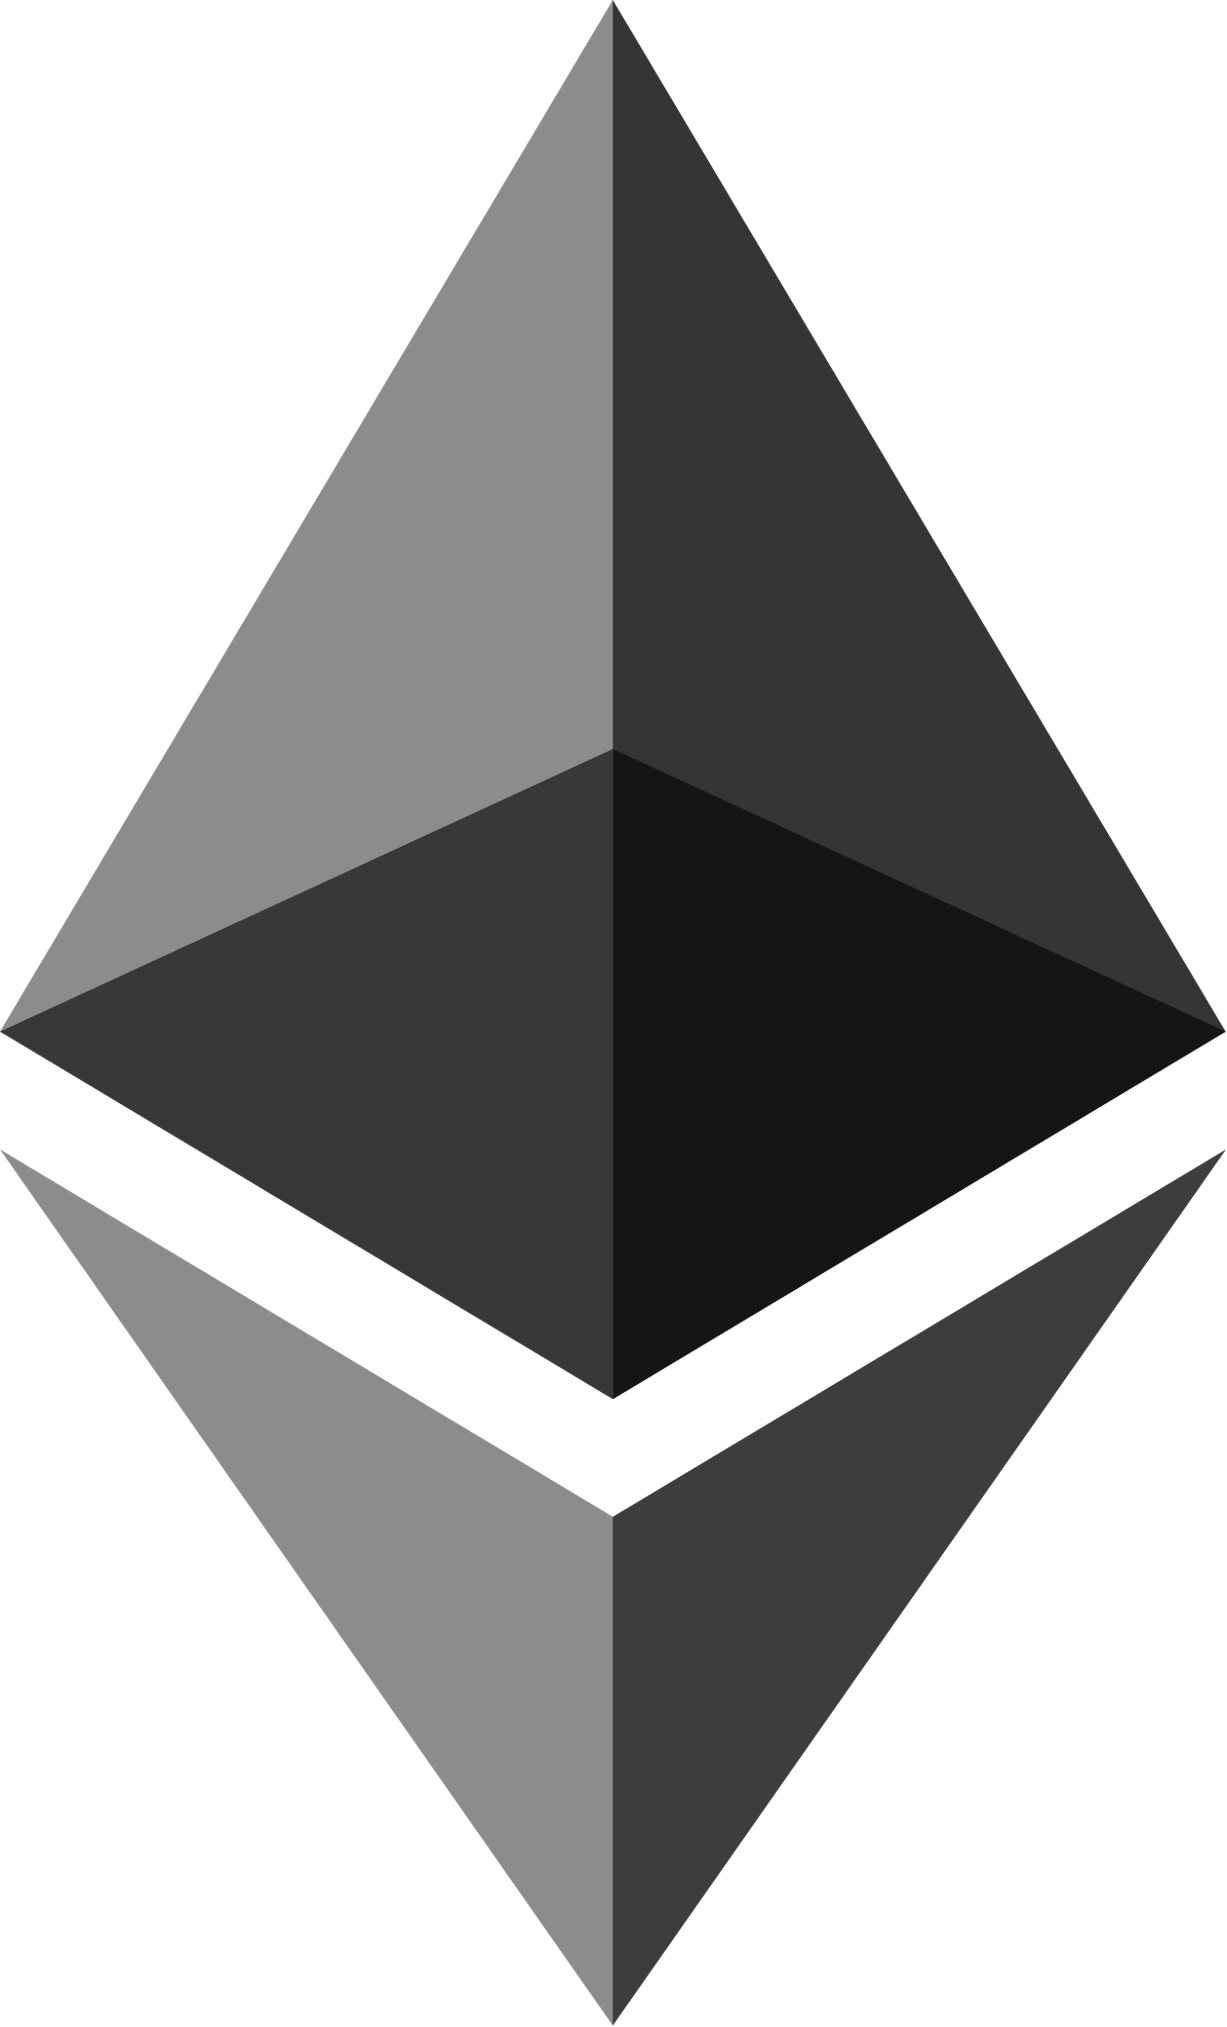
\includegraphics[width=0.05\textwidth]{ETH.png} & Ethereum & ETH & \$ 149 bn & 2\\
\\

\includegraphics[width=0.1\textwidth]{XRP.png} & XRP & XRP & \$ 20 bn & 7\\
\\

\includegraphics[width=0.1\textwidth]{LTC.png} & Litecoin & LTC & \$ 6 bn & 13\\
\\
\hline
\end{tabular}
\caption{\label{tab1} Cryptocurrencies. Quelle 2}
\end{table}


Besides these single cryptocurrencies, we also consider a cryptocurrency index. By looking at an index, we can replicate the cryptocurrency market as a whole and abstract from indiosyncratic risks of single currencies. The index that was considered is the CMC Crypto 200 Index by Solactive. The CMC Crypto 200 Index tracks the price movementes of the top 200 cryptocurrencies by market capitalization. It was launched at year end 2018 and is calculated and distributed by Solactive AG. The index is published in USD. The calculation of the index price is conducted on a daily basis (Quelle 1). As of November 2022, the four cryptocurrencies analyzed in this paper (Bitcoin, Etherium,  XRP and Litecoinwere) were within the 13 cryptocurrencies with the highest market capitalization and therefore also part of the CMC Crypto 200 (see Table 1).





\\

Quelle 1: https://www.solactive.com/wp-content/uploads/2019/04/Solactive-Index-Guideline-CMC200.pdf
Quelle 2: https://www.coingecko.com/



\section{Dataset description}
Here you can provide, if applicable, information about the dataset(s) whose creation, collection, management, access, processing or analysis have been discussed in this paper, following this schema:
\paragraph{Object name} Typically the name of the file or file set in the repository.
\paragraph{Format names and versions} E.g., ASCII, CSV, Autocad, EPS, JPEG, Excel, SQL, etc.
\paragraph{Creation dates} The start and end dates of when the data was created (YYYY-MM-DD).
\paragraph{Dataset creators} Please list anyone who helped to create the dataset (who may or may not be an author of the data paper), including their roles (using and affiliations).
\paragraph{Language} Languages used in the dataset (i.e., for variable names etc.).
\paragraph{License} The open license under which the data has been deposited (e.g., CC0). 
\paragraph{Repository name} The name of the repository to which the data is uploaded. E.g., Figshare, Dataverse, etc. 
\paragraph{Publication date} If already known, the date in which the dataset was published in the repository (YYYY-MM-DD).

\section{Method}
The goal of this paper is to assess wheter there is any connection between the 10 year treasury yiel and cryptocurrencies. To detect a potential connection we relied on classical statistical measures: covariance and correlation.

\subsection{Covariance}
The covariance is a measure to relate the movement of two random variables. A positive covariance indicates that the two variables move in the same direction. A negative covariance means that the variables move inversely, meaning that if one increases, the other one will decrease and vice versa. Therefore, covariance measures the direction of a relation. The covariance is given by the following formula:
\begin{center}
   \large $cov_{x,y}=\frac{\sum_{i=1}^{N}(x_{i}-\bar{x})(y_{i}-\bar{y})}{N-1}$
\end{center}
By calculating the Covariance we can examine the direction of a potential relationship between the 10 year treasury yield and the cryptocurrencies.

\subsection{Pearson's Correlation}
Similarly to the covariance, also the correlation is a measure for relationship. The correlation measures the strength of a relationship. The correlation coefficient lives on the inverval between negative one and one. The higher the absolute value, the stronger is the observed relationship. A correlation of zero indicates no relationship between the observed variables. Therefore, this measure is very intersting for our resarch question. Depending on the correlation we can assess how strong the relationship between the 10 year treasury yield and the cryptocurrencies is (if any).
First, we assess the Pearson's correlation. The Pearson coefficient will will measure any linear relationships between the variables. There is a linear relationship when a change in the first variable causes a proportional change in the second variable.


\subsection{Spearman's Correlation}
As we have seen above, the Pearson's correlation has its limits. Namely it is limited at measuring linear relationships. We therefore also introduce a second correlation measure, called the Spearman's correlation. The Spearman’s correlation coefficient extends the concept to non-linear, monotonic functions. Simply put, monotonic functions are functions that do not change direction but can have different steepness throughout. 




\section{Results and discussion}


#The correlation between the 10yr treasury yield and other cryptocurrencies is very weak and shows negligible correlation.
#The interesting fact is if we compare BTC to other cryptos we see very high positive correlation.


#As seen from the results the correlation between the 10yr treasury yield and other cryptocurrencies is very weak
#For them to be at least moderatily correlated, the Spearman correlation coefficient would have to be greater than 0.40 in absolute terms.
#We conclude that there is no significant correlation between interest rate hikes and cryptocurrency exchange rates

\section{Implications/Applications}
Provide information about the implications of this research and/or how it can be applied.

\newpage


\bibliographystyle{johd}
\bibliography{bib}

\end{document}